\documentclass[10 pt,usenames,dvipsnames, oneside]{article}
\usepackage{../../../modelo-ensino-medio}



\begin{document}

\begin{center}
  \begin{minipage}[l]{3cm}

\includegraphics[width=2cm]{logo}    
\end{minipage}\hfill
\begin{minipage}[r]{.8\textwidth}
 {\Large \scshape Atividade: Várias curvas}  
\end{minipage}
\end{center}
\vspace{.2cm}

\ifdefined\prof
%Habilidades da BNCC
\begin{objetivos}
\item \textbf{EM13MAT304} Resolver e elaborar problemas com funções exponenciais nos quais é necessário compreender e interpretar a variação das grandezas envolvidas, em contextos como o da Matemática Financeira e o do crescimento de seres vivos microscópicos, entre outros. 
\end{objetivos}

%Caixa do Para o Professor
\begin{goals}
%Objetivos específicos
\begin{enumerate}
\item Deduzir expressões algébricas para funções exponenciais a partir de gráficos.
\end{enumerate}

\tcblower

%Orientações e sugestões
\begin{itemize}
\item Peça aos estudantes que compartilhem com a turma sobre os raciocínios que tiveram para deduzir as expressões.

\item Após a discussão peça para os estudantes proporem desafios para os colegas.
\end{itemize}
\end{goals}

\bigskip
\begin{center}
{\large \scshape Atividade}
\end{center}
\fi

Abaixo, todos os gráficos são de funções exponenciais. Escreva expressões para cada uma delas.

\begin{enumerate}

\item{}
\adjustbox{valign=t}
{
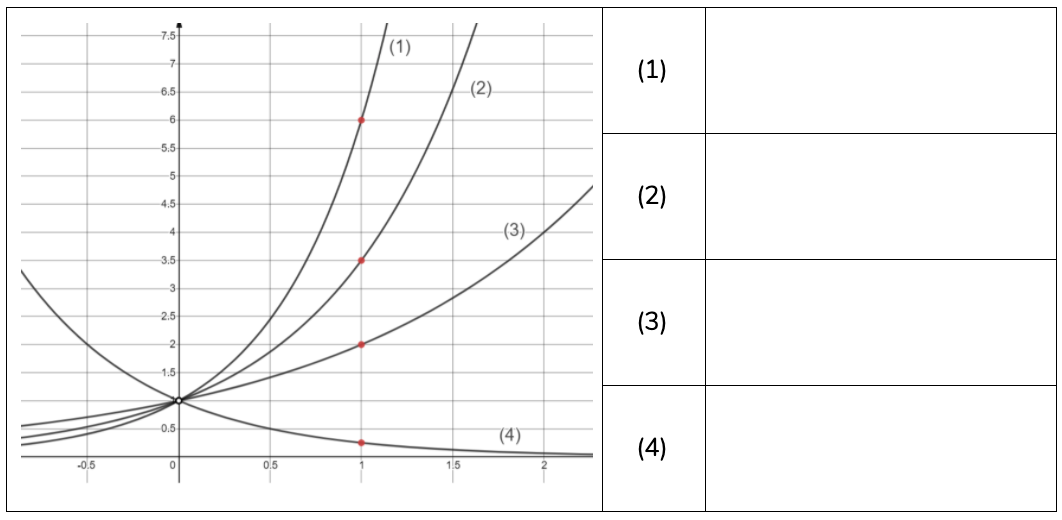
\includegraphics[width=350bp]{exponenciais.png}
}


\item{}

\adjustbox{valign=t}
{
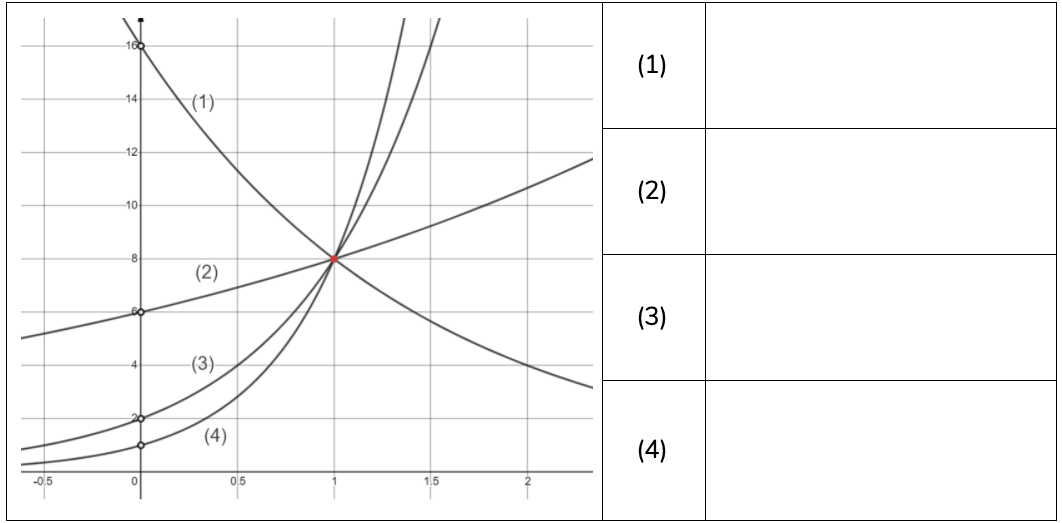
\includegraphics[width=350bp]{exponenciais1.png}
}


\item{}

\adjustbox{valign=t}
{
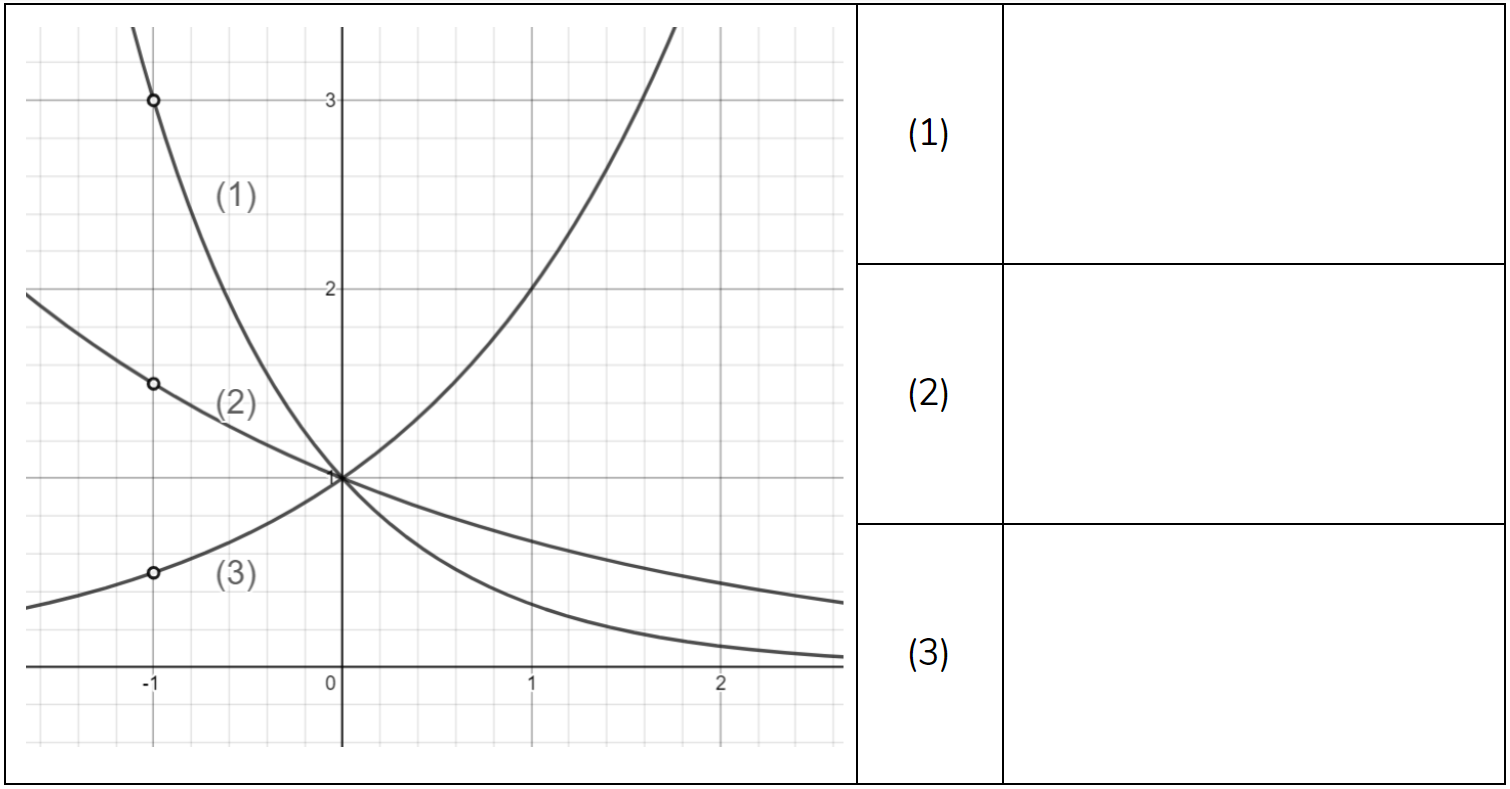
\includegraphics[width=350bp]{exponenciais3.png}
}


\end{enumerate}

\ifdefined\prof
\begin{solucao}

\begin{enumerate}

\item \begin{enumerate}[label=(\arabic*)]
\item $y=6^x$; 
\item $y=3{,}5^x$;
\item $y=2^x$;
\item $y=0{,}25^x$.
\end{enumerate}

\item \begin{enumerate}[label=(\arabic*)]
\item $y=16 \cdot 0{,}5^x$; 
\item $y=6\cdot \left(\frac 43\right)^x$; 
\item $y=2\cdot 4^x$; 
\item $y=8^x$.
\end{enumerate}

\item \begin{enumerate}[label=(\arabic*)]
\item $y=\left(\frac 13\right)^x=3^{-x}$; 
\item $y=\left(\frac 23\right)^x=1.5^{-x}$; 
\item $y=2^x$.
\end{enumerate}


\end{enumerate}

\end{solucao}
\fi

\end{document}